\ylDisplay{Sfäär} % Ülesande nimi
{Andre Sääsk} % Autor
{lahtine} % Voor
{2005} % Aasta
{G 6} % Ülesande nr.
{5} % Raskustase
{
% Teema: Dünaamika
\ifStatement
Üks osa Pariisi Cité des Sciences teadusmuuseumi kompleksist --- La Géode --- kujutab endast hiigelsuurt sfääri raadiusega $R = \SI{18}{m}$, mille sees asub maailma suurim kinoekraan (vt joonist). Hoonet väljastpoolt imetlev uudishimulik koolipoiss otsustab tabada selle hoone tipp-punkti tennisepalliga. Kui suure minimaalse kiirusega $v$ peaks ta palli viskama, et palli liikumise trajektoor lõikuks hoone välispinnaga vaid ühes punktis --- hoone tipp-punktis --- ja see oleks ühtlasi ka palli liikumise trajektoori kõrgeimaks punktiks? Pall alustab liikumist kõrgusel $h = \SI{1,5}{m}$.

\begin{center}
	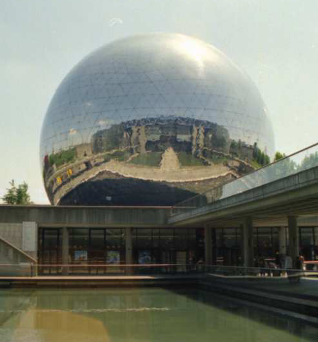
\includegraphics[width=0.5\linewidth]{2005-lahg-06-yl}
\end{center}
\fi


\ifHint
Kriitilise kiiruse korral on palli trajektoori kõverusraadius sfääri tipp punktis võrdne sfääri raadiusega. See tähendab, et pallile mõjuva raskuskiirenduse tasakaalustab kesktõmbe kiirendus $v^2/R$.
\fi


\ifSolution
Kuna küsitakse ainult minimaalset vajalikku kiirust (arvväärtust), siis ei pea me leidma ei viske nurka ega viske kohta. Vertikaalsuunalise kiiruse komponendi viske hetkel leiame energia jäävuse seadusest:
\[
\frac{m v_{y 0}^{2}}{2}=m g \Delta h=m g(2 R-h) \quad \Rightarrow \quad v_{y 0}=\sqrt{2 g(2 R-h)}.
\]
Horisontaalsuunalise kiiruse komponendi leiame tingimusest, et sfääri ülemises punktis peab olema pallile mõjuv kesktõmbe kiirendus $v^2/R$ võrdne pallile mõjuva raskuskiirendusega. Kuna sfääri ülemises punktis on $v_y = 0$, siis $v = v_x$. Kuna õhu takistust me ei arvesta, siis $v_x = v_{x0}$ (kiiruse horisontaalsuunaline komponent ei muutu lennu ajal). Seega
\[
\frac{v_{x 0}^{2}}{R}=g \quad \Rightarrow \quad v_{x 0}=\sqrt{g R}.
\]
Teades kahte kiiruse komponenti, on lihtne leida kogu kiiruse viske hetkel:
\[
v=\sqrt{v_{x 0}^{2}+v_{y 0}^{2}}=\sqrt{g R+2 g(2 R-h)}=\sqrt{g(5 R-2 h)} \approx \SI{29}{m/s}.
\]

\vspace{0.5\baselineskip}

\emph{Alternatiivne lahendus}

Läheneme ülesandele matemaatiliselt. Meil on ringjoon, parabool ning nende puutepunkt. Lahendades nende võrrandid puutepunkti leidmiseks peame saama ainult ühe lahendi, sest visatud pall ei tohi läbida kuplit. Koordinaatide alguspunkti paneme kera keskpunkti, $y$-telg on suunatud vertikaalselt üles, $x$-telg --- horisontaalselt viske suunas.

Ringjoone võrrand
\[
x^2 + y^2 = R^2.
\]
Parabooli võrrand
\[
y = ax^2 + bx + c.
\]

\begin{center}
	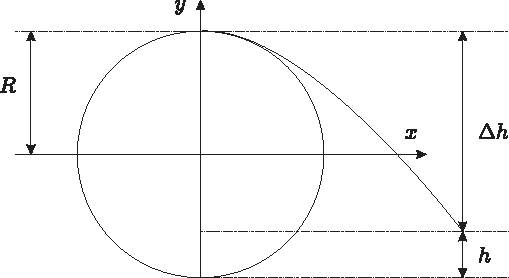
\includegraphics[width=0.8\linewidth]{2005-lahg-06-lah}
\end{center}

Sümmeetriast $y$-telje suhtes on $b = 0$, palli ja kupli kokkupuutepunkti teades on $x = 0$ puhul $y = R$ (vt joonist). Seega $c = R$ ja parabooli võrrand omandab kuju:
\[
y = ax^2 + R.
\]
Nüüd tuleb ühest võrrandist tundmatu asendada teise. Olgu selleks parabooli võrrandi $y$, mille asendame ringjoone võrrandisse:
\[
x^{2}+\left(a x^{2}+R\right)^{2}=R^{2},
\]
\[
x^{2}+a^{2} x^{4}+2 a R x^{2}+R^{2}=R^{2},
\]
\[
x^{4}+\left(\frac{2 a R+1}{a^{2}}\right) x^{2}=0.
\]
Lahendades selle võrrandi, saame kolm lahendit:
\[
x=0, \quad x=\pm \sqrt{-\frac{2 a R+1}{a^{2}}}.
\]
Meile sobib ainult esimene lahend, sest teised kaks on imaginaarsed. Seega
\[
2aR + 1 = 0 \quad\Rightarrow\quad a = - \frac{1}{2R}.
\]
Nüüd on paras aeg analüüsida kiiruse komponente. Vaatleme kõigepealt kiiruse vertikaalset komponenti. Energia jäävuse seadusest teame, et palli kineetiline energia viske alguses muundub palli potentsiaalseks energiaks trajektoori tipppunktis:
\[
\frac{m v_{0 y}^{2}}{2}=m g \Delta h=m g(2 R-h) \quad\Rightarrow\quad v_{0 y}=\sqrt{2 g(2 R-h)}.
\]
Teisest küljest, kiiruse võrrandist teame, et
\[
v_{0 y}=g \Delta t \quad \Rightarrow \quad \Delta t=\frac{v_{0 y}}{g}=\frac{\sqrt{2 g(2 R-h)}}{g}.
\]
Seega lennuaeg on paika pandud viskekohta arvestamata. Analüüsime parabooli võrrandit viskekohas
\[
-R + h = ax^2 + R \Rightarrow x^2 = \frac{h-2R}{a}.
\]
Lennuaeg on juba määratud, seega mida väiksem on $x$, seda väiksema kiirusega võib pall läbida vahemaad viskekohast nullpunkti vaadelduna $x$-teljel. Seega peab $a$ olema võimalikult suur. Asendades suurima $a$ saab
\[
x=\sqrt{\frac{h-2 R}{-1 / 2 R}}=\sqrt{2 R(2 R-h)}.
\]
Kiiruse $x$-teljeline komponent teepikkuse ja aja suhtena on
\[
v_{0 x}=\frac{\Delta x}{\Delta t}=\frac{g \sqrt{2 R(2 R-h)}}{\sqrt{2 g(2 R-h)}}=\sqrt{\frac{g^{2} R}{g}}=\sqrt{g R}.
\]
Liites komponendid saame minimaalse viske kiiruse:
\[
v=\sqrt{v_{0 x}^{2}+v_{0 y}^{2}}=\sqrt{g R+2 g(2 R-h)}=\sqrt{g(5 R-2 h)} \approx \SI{29}{m/s}.
\]
Antud lahendus on hea näide sellest, kui pikk ja keeruline võib olla ülesande matemaatiline lahendus võrreldes füüsikalisega.
\fi
}